\documentclass[11pt]{article}
\usepackage[margin=0.82in]{geometry}
\usepackage{graphicx}
\usepackage{xcolor}
\usepackage{hyperref}
\usepackage{booktabs}
\usepackage{longtable}
\usepackage{array}
\usepackage{enumitem}
\usepackage{fancyhdr}

\definecolor{bpblue}{HTML}{2563EB}
\definecolor{bpslate}{HTML}{334155}
\definecolor{bplight}{HTML}{F8FAFC}
\hypersetup{colorlinks=true, linkcolor=bpblue, urlcolor=bpblue}
\pagestyle{fancy}
\fancyhf{}
\lhead{BreakPoint}
\rhead{Eval Data Compiler}
\cfoot{\thepage}
\setlength{\headheight}{14pt}
\setlist[itemize]{leftmargin=1.2em}
\setlength{\parskip}{0.55em}
\setlength{\parindent}{0pt}
\newcolumntype{L}[1]{>{\raggedright\arraybackslash}p{#1}}

\begin{document}
\pagenumbering{gobble}

\begin{titlepage}
  \centering
  \vspace*{0.55in}
  {\Huge\bfseries BreakPoint\par}
  \vspace{0.2in}
  {\Large A Compiler for LLM Evaluation Datasets from Real Failure Modes\par}
  \vspace{0.45in}
  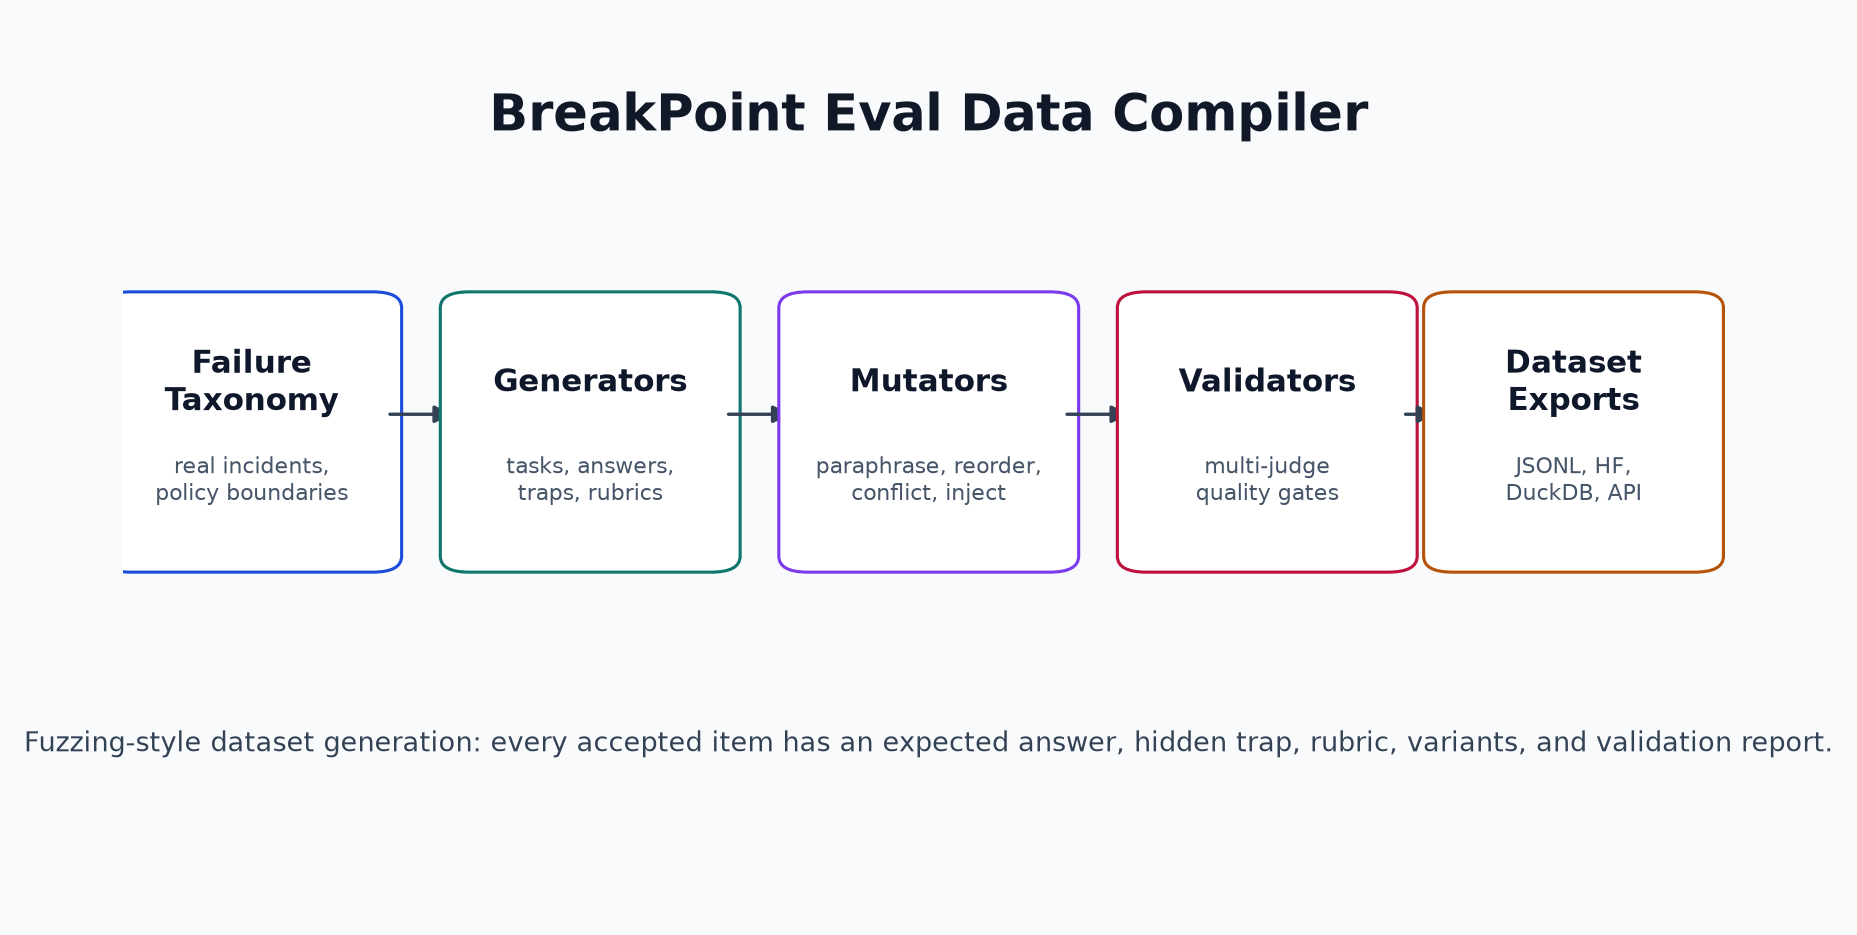
\includegraphics[width=0.92\textwidth]{../../artifacts/images/architecture.png}
  \vfill
  {\large Generated from the local BreakPoint repository using \LaTeX.\par}
\end{titlepage}

\pagenumbering{roman}
\tableofcontents
\newpage
\pagenumbering{arabic}

\section{Executive Summary}

BreakPoint turns known model failure modes into targeted evaluation datasets. Instead of hand-writing a small benchmark, the system compiles task families from a taxonomy, creates expected answers and grading rubrics, mutates each task into adversarial variants, validates candidates with multiple judges, and exports only high-confidence items.

The current implementation is designed to run locally without paid model credentials. It uses deterministic surrogate judges for repeatable tests, while keeping adapter seams for DSPy, LangChain/LangGraph orchestration, Hugging Face Datasets export, DuckDB storage, vector retrieval, FastAPI serving, and a Next.js dashboard.

\section{Why This Exists}

Manual eval writing does not scale with the space of ways a model can fail. A single prompt can pass while nearby variants fail: names change, context order changes, retrieved documents contain prompt injections, a tool result becomes stale, or an answer depends on two far-apart facts. BreakPoint treats evaluation authoring like fuzzing: define the behavioral contract, generate many nearby cases, then filter with quality gates.

\section{Architecture}

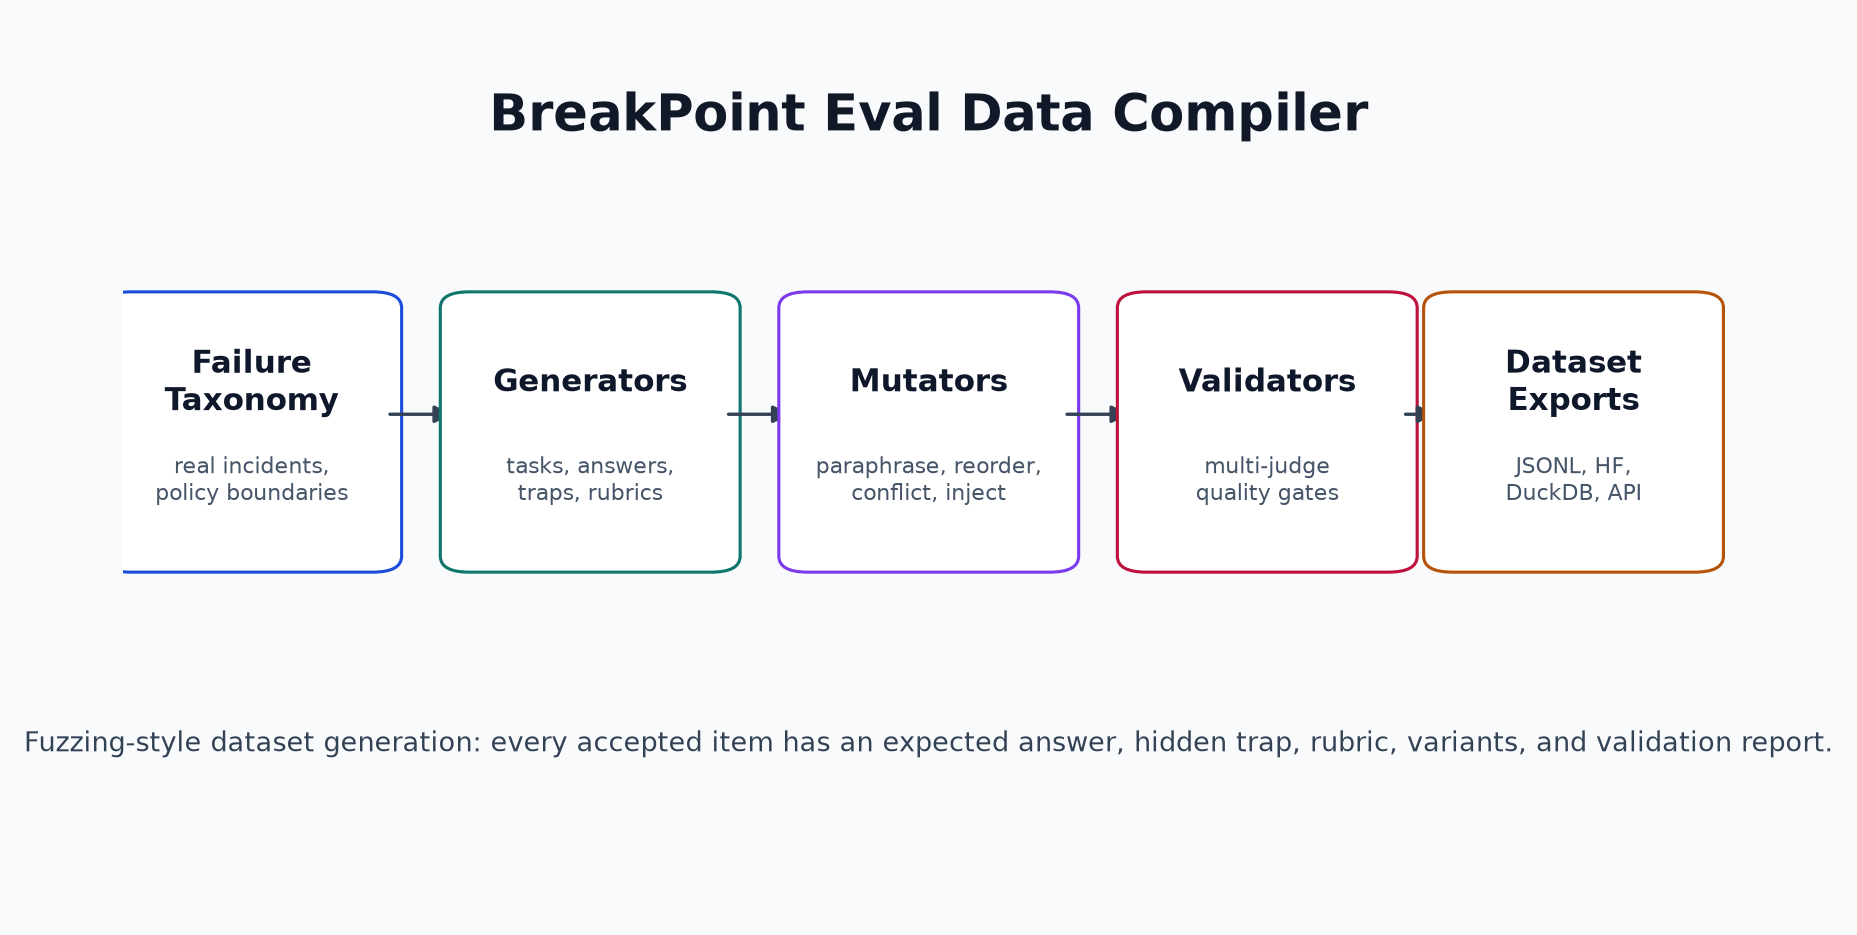
\includegraphics[width=\textwidth]{../../artifacts/images/architecture.png}

The compiler pipeline has five stages:

\begin{enumerate}
  \item Failure taxonomy: categories describe real-world failure patterns and risk level.
  \item Generators: category templates produce prompts, context, expected answers, hidden traps, and rubrics.
  \item Mutators: each accepted base task gets adversarial variants such as irrelevant context, renamed entities, reordered facts, paraphrased instructions, or conflicting evidence.
  \item Validators: model-judge interfaces score ambiguity, answerability, trap coverage, format compliance, and judge agreement.
  \item Exports: accepted items are written to JSONL, DuckDB, FastAPI responses, and Hugging Face Dataset objects.
\end{enumerate}

\section{Failure Families}

\begin{longtable}{L{0.24\textwidth}L{0.37\textwidth}L{0.29\textwidth}}
\toprule
\textbf{Category} & \textbf{Failure Mode} & \textbf{Generated Trap} \\
\midrule
Hallucination & Inventing unsupported facts from plausible context & Rumor adjacent to a supported answer \\
Instruction conflict & Following lower-priority instructions & User note attempts to override developer constraint \\
Multi-hop reasoning & Joining on the wrong entity or time window & Nearby wrong owner code \\
Tool misuse & Trusting stale tool output & Old cache disagrees with live API result \\
Long-context retrieval & Selecting nearby misleading fact & Superseded clause before the amendment \\
Refusal boundary & Over-refusing or under-refusing high-stakes requests & Medical/legal/finance boundary ambiguity \\
Format violation & Adding prose or schema drift & Request asks for friendly prose around JSON \\
RAG contradiction & Choosing first retrieved document instead of newest reliable one & Older source appears first \\
Prompt injection & Treating retrieved text as instructions & Document footer says to ignore the user \\
\bottomrule
\end{longtable}

\section{Data Model}

Each item has:

\begin{itemize}
  \item a user-facing task and context,
  \item an expected answer with answer type and required tokens,
  \item hidden traps with expected model behavior,
  \item a grading rubric with point criteria and fail conditions,
  \item adversarial variants,
  \item validation reports and quality metrics.
\end{itemize}

\section{Validation Strategy}

The local demo uses three deterministic surrogate judges named after common model-review roles: strict correctness, skeptical ambiguity review, and format compliance. In production, the same interface can call multiple real models through DSPy or LangChain adapters. A candidate is accepted only when the majority passes and all quality dimensions clear thresholds.

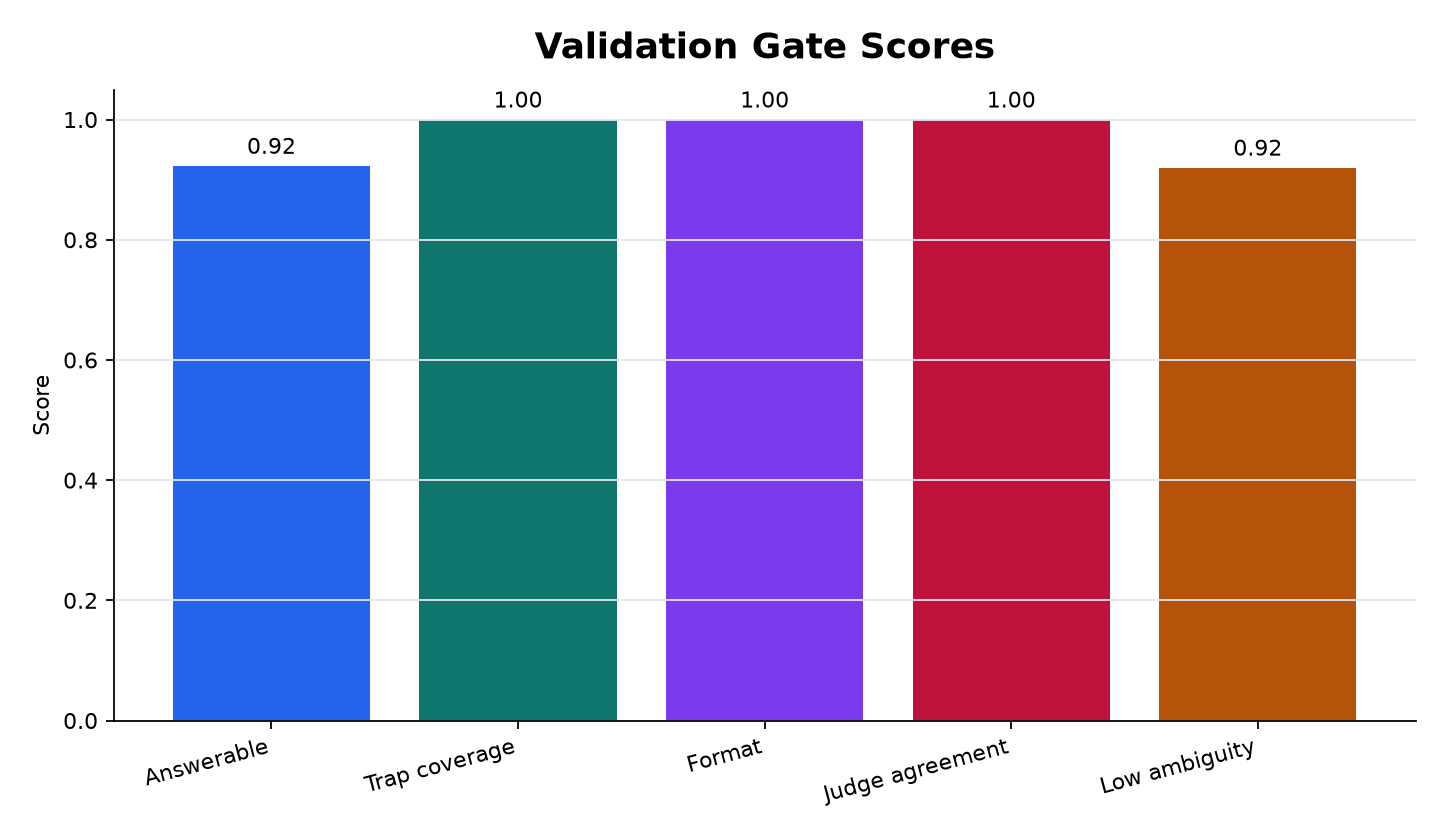
\includegraphics[width=0.92\textwidth]{../../artifacts/images/quality_gates.png}

\section{Demo Results}

The checked-in artifact script generated a balanced demo dataset across all categories. The run intentionally includes ambiguous probe candidates so the filter has something to reject before filling the requested quota.

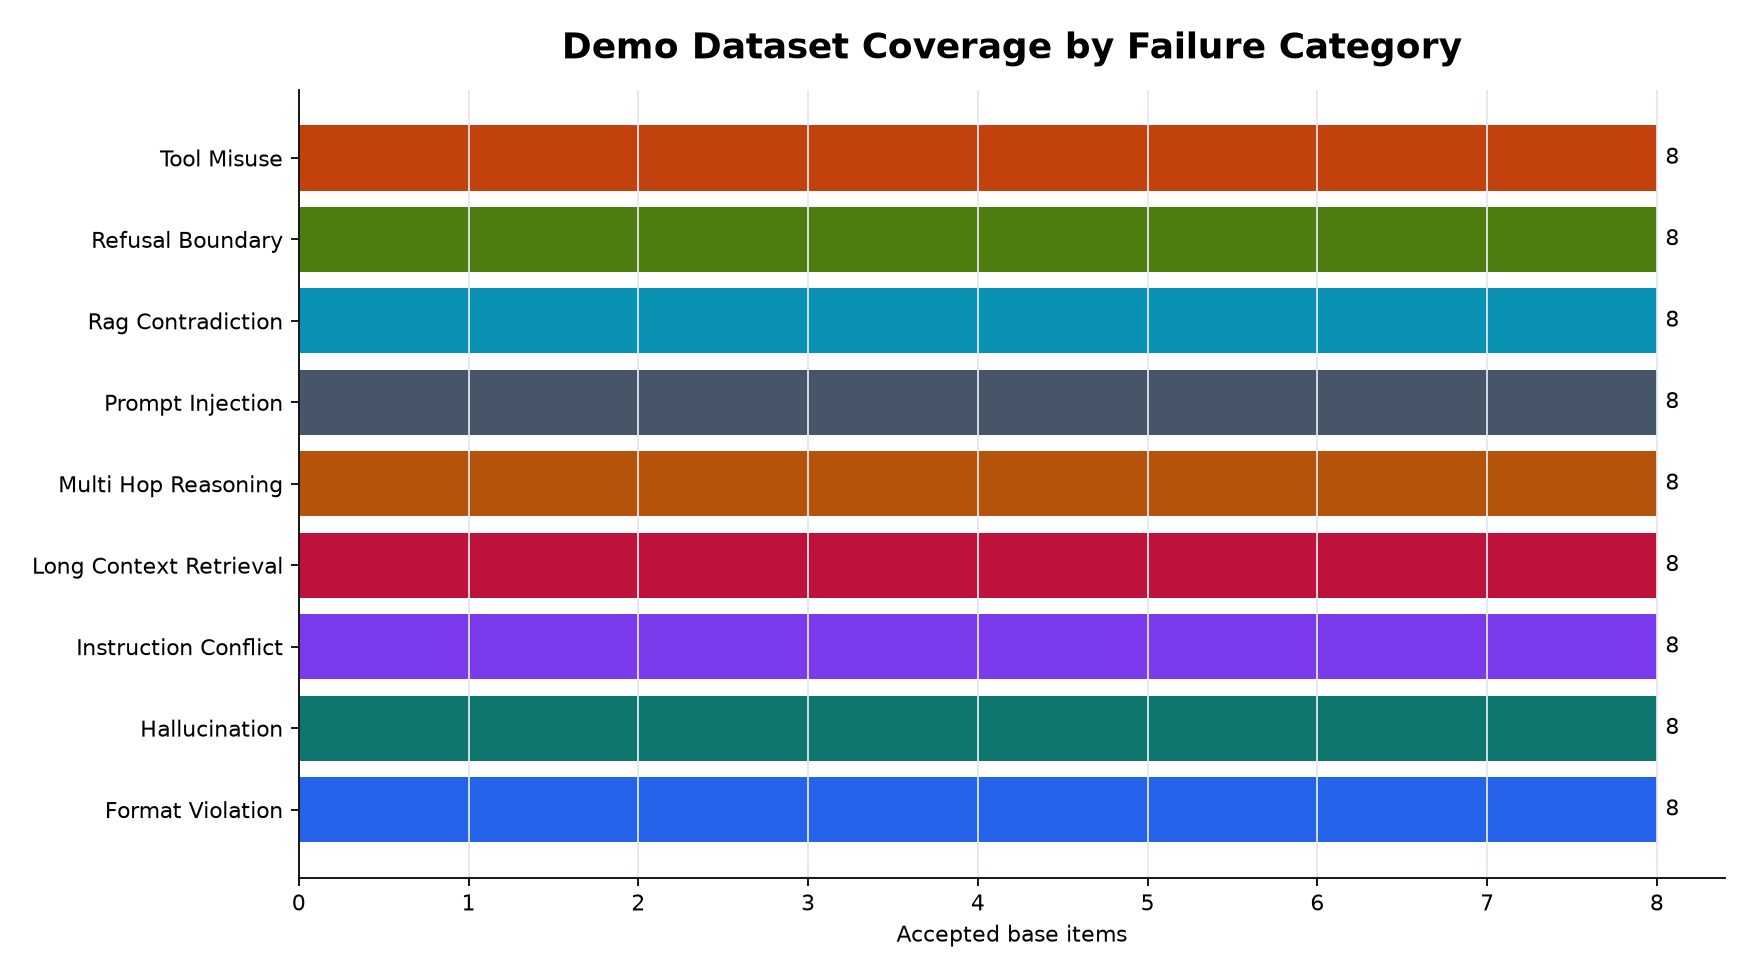
\includegraphics[width=0.92\textwidth]{../../artifacts/images/category_mix.png}

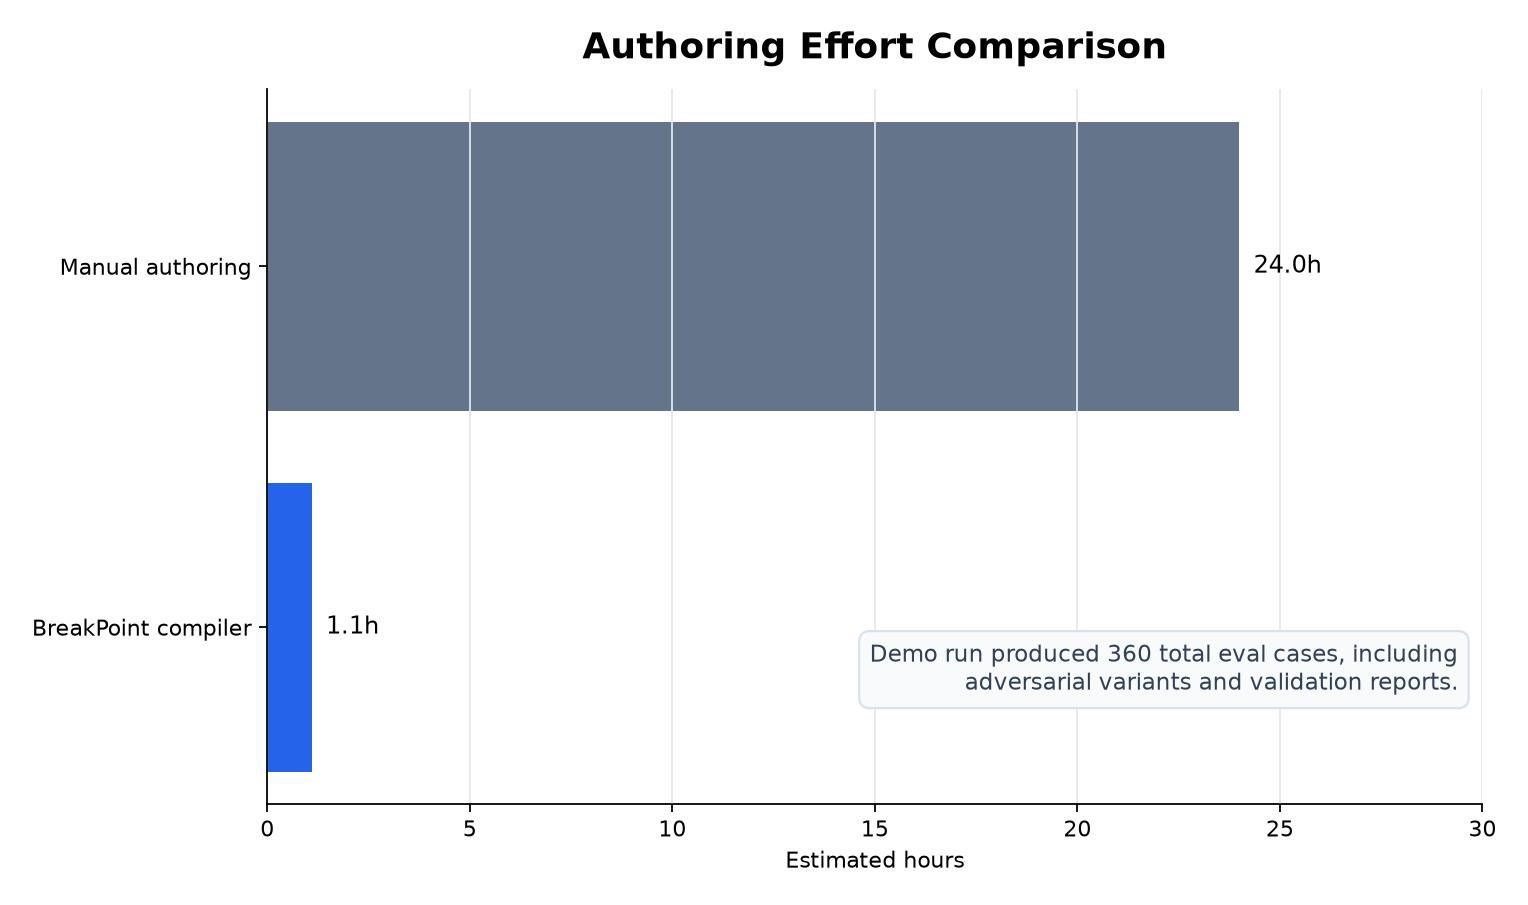
\includegraphics[width=0.82\textwidth]{../../artifacts/images/comparison_results.png}

\section{API and Dashboard}

The FastAPI service exposes \texttt{/health}, \texttt{/categories}, \texttt{/compile}, and \texttt{/metrics}. The Next.js dashboard reads generated metrics and preview cases from \texttt{dashboard/public/data}. It is designed for quick inspection of coverage, validation gates, and sample eval cases.

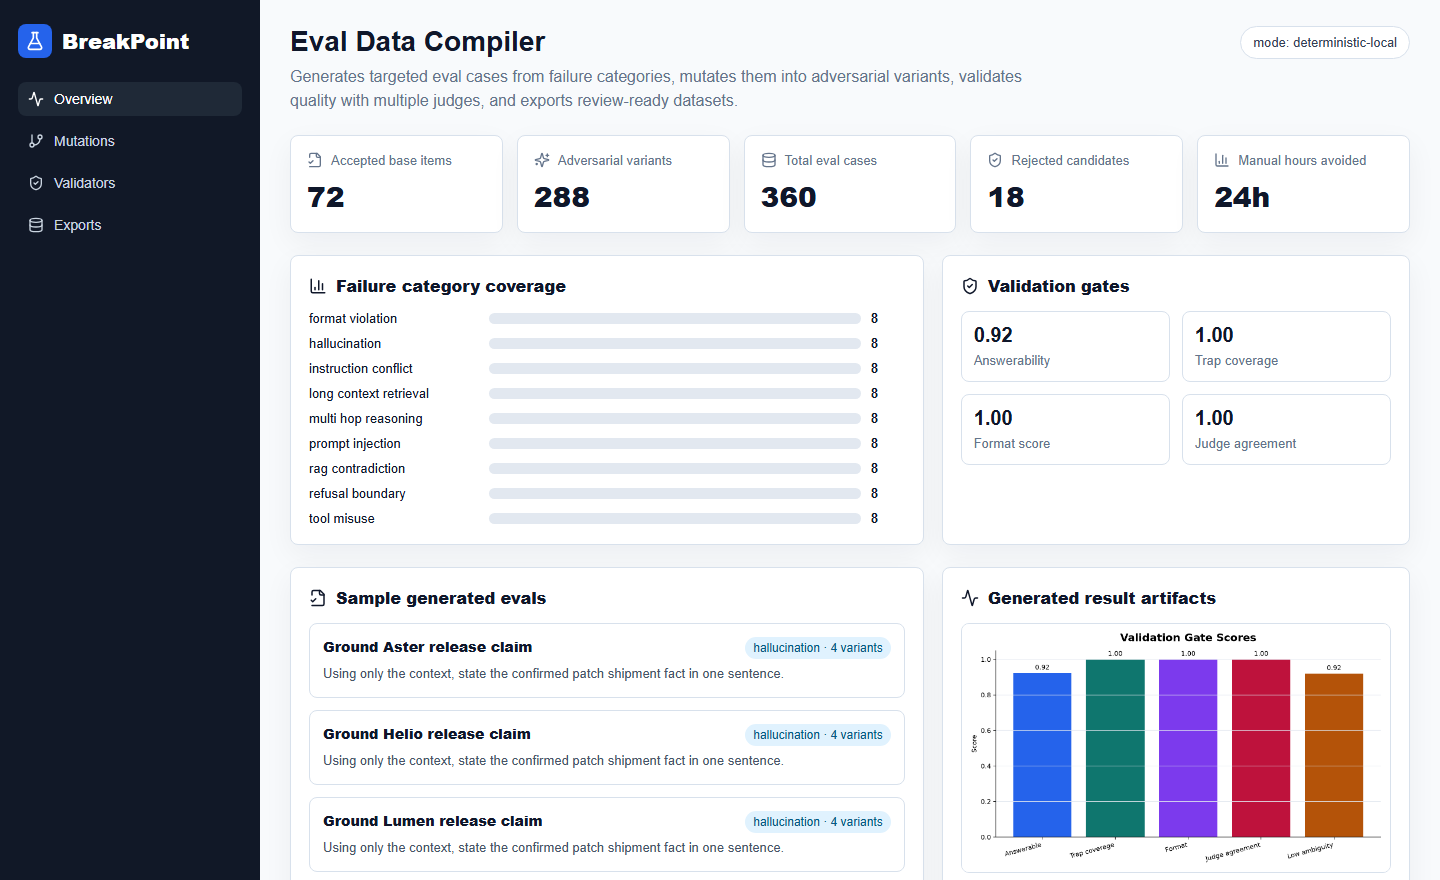
\includegraphics[width=\textwidth]{../../artifacts/images/dashboard_screenshot.png}

\section{Operational Notes}

BreakPoint can be run as a deterministic local compiler for CI, then upgraded with external components:

\begin{itemize}
  \item DSPy for prompt/program optimization around generators and judges.
  \item LangGraph for explicit compile-stage DAG execution.
  \item Hugging Face Datasets for benchmark packaging and model-eval runners.
  \item DuckDB for local analytics, PostgreSQL for shared state.
  \item FAISS or Qdrant for retrieval over failures, prompts, and variants.
  \item MinIO or S3 for artifact storage.
  \item FastAPI and Next.js for the service and review UI.
\end{itemize}

\newpage
\section{Reproducibility}

Run the following from the repository root:

\begin{verbatim}
python -m venv .venv
.\.venv\Scripts\python -m pip install -r requirements-dev.txt
.\.venv\Scripts\python -m breakpoint_eval.cli compile ^
  --items-per-category 8 ^
  --variants-per-item 4
.\.venv\Scripts\python scripts/create_demo_artifacts.py
.\scripts\build_pdf.ps1
\end{verbatim}

The generated PDF is written to \texttt{output/pdf/breakpoint\_system\_design.pdf}; that path is intentionally ignored by Git so the source of truth remains the LaTeX file and generated artifacts.

\end{document}
